\chapter{Experimental design and apparatus}
\label{ch:experiment}
\graphicspath{{Chapter-Experiment/figures/}}

\section{Scattering experiments}

\subsection{History and motivation}
The first modern scattering experiments were the Geiger-Marsden experiments in the early 1910s, in which the Rutherford scattering of alpha ($\alpha$) particles by gold foil was observed \cite{Rutherford:1911zz}.
While most $\alpha$ particles passed through the foil with little deflection, a small fraction of them were deflected to extreme angles (\cref{fig:rutherford}).
This result provided evidence that electric charge within the foil was not distributed uniformly, but localized in very small clusters -- the nuclei of the gold atoms.
\begin{figure}[t]
  %% https://www.chegg.com/homework-help/questions-and-answers/rutherford-s-experiment-studied-deflection-scattering-ofalpha-particles-known-helium-nucle-q458296
  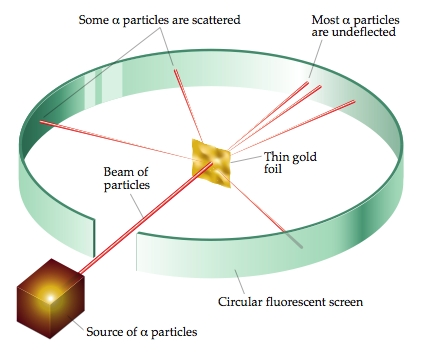
\includegraphics{BLB-1070873-Rutherford_v2.jpg}
  \caption{Rutherford scattering of alpha particles by gold foil, demonstrating the existence of the atomic nucleus.}
  \label{fig:rutherford}
\end{figure}

With elementary quantum mechanics, this type of elastic scattering can be understood more precisely.
In the Born approximation, which is essentially the weak-potential limit, the quantum amplitude $f$ of a particle with incoming momentum $\mathbf{p}_{i}$ scattering elastically off a target potential $V(\mathbf{x})$ with outgoing momentum $\mathbf{p}_{f}$ is proportional to the Fourier transform of the potential:

\begin{equation}
  f\left(\mathbf{p}_f ; \mathbf{p}_i\right) \propto - \int d^3 x \, V(\mathbf{x}) e^{-i \Delta \mathbf{p} \cdot \mathbf{x}}
  \label{eq:born}
\end{equation}
where $\Delta \mathbf{p} \equiv \mathbf{p}_f - \mathbf{p}_i$ is the momentum transferred to the projectile particle.
The differential scattering cross-section $d\sigma/d\Omega$ (the scattering probability density per unit area) is given by the square of the quantum amplitude, so it is proportional to the squared magnitude of the Fourier transform of the potential.

\begin{equation}
  \frac{d\sigma}{d\Omega} \propto \left| \int d^3 x \, V(\mathbf{x}) e^{-i \Delta \mathbf{p} \cdot \mathbf{x} / \hbar} \right|^2 = \left| \tilde{V}(\mathbf{\Delta \mathbf{p}}) \right|^2
\end{equation}
Because the net momentum transfer is constrained by the relative momentum between projectile and target, larger momentum -- or equivalently, higher energy -- is required to probe the finer structure of the target.
This correspondence between center-of-mass energy and the spatial resolution of the probe remains valid even for inelastic collisions and strong interactions.
The required energy to probe a distance scale can be estimated with dimensional analysis.
To resolve the structure of a target down to a distance scale $l$, the center-of-mass energy $E$ is

\begin{equation}
E = \frac{\hbar c}{l} \approx \frac{0.2 \GeV \fm}{l} \; .
\end{equation}
Resolving individual atoms requires collisions with energy of order \keV, resolving the nucleus requires at least \MeV\ scale energies, and resolving sub-nucleic structure requires collisions of at least order \GeV.

\subsection{Accelerator physics}

The energy of a beam collision is described by the Lorentz-invariant quantity $\sqrt{s}$ where $s = (p_a + p_b)^2$ with $p_a$ and $p_b$ being the four-momenta of the beam particles.
In the center-of-momentum frame, $\sqrt{s}$ is the total energy of the collision.
The beam energy in heavy ion and proton-ion collisions is normalized by the mass of the nucleus.
In symmetric ion collisions with mass number $A$ this energy per nucleon is $\sqrt{s_\mathrm{NN}} = A^{-1} \sqrt{s}$.

In a fixed-target experiment using target particles of mass $m_t$ and a projectile beam with particles of rest mass $m_p$ and energy $E$, the center-of-momentum energy $\sqrt{s}$ is given by
\begin{equation}
\sqrt{s} = \sqrt{(m_t+m_p)^2 + 2 m_t (E - m_p)} \; ,
\end{equation}
which scales with the square root of the beam energy even for large energies.
On the other hand, if two beams are accelerated and directed into each other, the center-of-momentum energy of each collision is
\begin{equation}
\sqrt{s} = \sqrt{(E_t + E_p)^2 - (|\mathbf{p}_t| - |\mathbf{p}_p|)^2} \; ,
\end{equation}
which scales linearly with the total energy, and is equal to $2E$ in the case where the beams are identical.
While fixed-target experiments were the first to be developed, they are not as efficient at reaching high energies as dual-beam colliders.
Modern high-energy experiments therefore accelerate two particle beams and generate collisions by intersecting the beams head-on.

\subsubsection{Accelerator designs}

\begin{figure}[t]
  %%  https://www.cyberphysics.co.uk/topics/atomic/Accelerators/LINAC/Linac.htm
  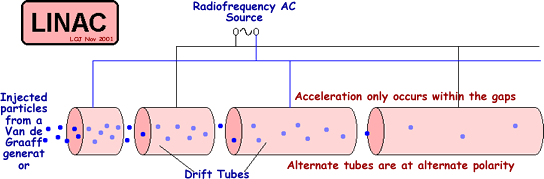
\includegraphics{LINAC.png}
  \caption{A linear accelerator.}
  \label{fig:linac}
\end{figure}

The most straightforward method to accelerate charged particles to high energies is to allow them to pass through a large voltage differential.
A large voltage can be produced, for instance, with a Van de Graaff generator \cite{PhysRev.43.149}.
The voltage differential is limited by the insulation breakdown, which in practice caps the energy of accelerated particles with charge $Ze$ to a few $Z \cdot\MeV$.
A modern \linac circumvents this issue by passing ions through a series of drift tubes with alternating positive and negative potentials (\cref{fig:linac}).
The drift tubes are constructed with conducting material, so they shield the ions traveling through them from external electric acceleration.
Between the drift tubes, however, strong electric fields are induced by the alternating potentials.
This voltage difference is oscillated with \rf and the apparatus is constructed such that ions injected at a given velocity can pass through each gap with acceleration in the forward direction.
The \ac{SLAC} hosts the largest linear accelerator, which began operation in 1966.
The 3 km long machine was capable of accelerating electrons and positrons to energies of up to 50 \GeV.
While this is several orders of magnitude higher than the energies accessible with a simple voltage differential, increasing the energy further requires proportional increases in the length of the accelerator, exacerbating technical difficulties in its placement, construction, and maintenance.

\begin{figure}[t]
 %% https://www.mpoweruk.com/figs/cyclotron.htm
  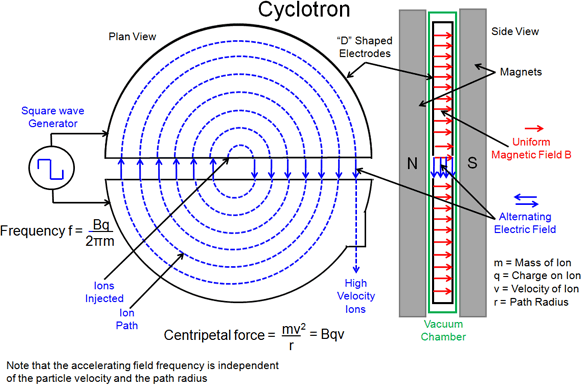
\includegraphics{cyclotron.png}
  \caption{A cyclotron.}
  \label{fig:cyclotron}
\end{figure}
The cyclotron is the next fundamental progression in accelerator technology.
Ions in a cyclotron are passed between two semi-cylindrical electrodes (``dees'') that are driven with an alternating voltage (\cref{fig:cyclotron}).
A large electromagnet keeps the particles traveling in a circular path contained within the dees.
At non-relativistic energies, the velocity of the ions is proportional to the radius of their path, so the time taken for one revolution is independent of the velocity.
If the voltage between the electrodes is oscillated with a frequency equal to the cyclotron resonance frequency $f_\textrm{cyclo} = q B / 2\pi m$, then ions are accelerated to higher energies with each pass between the dees.
At a fixed radius (and therefore fixed energy), the ion beam is allowed to exit the cyclotron.
Classically, the kinetic energy is proportional to the square of the radius, inviting a comparison to a hypothetically coiled \linac.
Relativistic energies can be attained with more sophisticated designs that vary either the frequency over time or the magnetic field with the radial position, but as the velocity approaches $c$ the energy is only linearly proportional to the radius:
\begin{align}
\label{eq:gyroradius}
E =& \; \frac{q B R c^2}{v}\\
\overrightarrow{{}_{v \rightarrow c}}& \; q B R c
\end{align}
This shows that the energies accessible from a circular accelerator are directly limited by the maximum strength of the magnetic field and the radius of the path.

The radius of a cyclotron design can only be increased so much before it becomes infeasible.
The synchrotron is a toroidal accelerator in which ion beams travel around the torus, turned by dipole magnets along the path.
Quadrupole and higher-multipole magnets are used to maintain the focus of the beam and make fine-tuning adjustments to the magnetic fields.
This layout does not permit particles to be accelerated from an arbitrarily small energy, so a synchrotron is generally filled with particles first accelerated from a \linac, and the ions are kept circling the path at the injection energy.
Once the beam pipe is filled, the energy of the ion beam is gradually increased by \rf cavities that oscillate to apply an acceleration to the particles.
The oscillation of the \rf cavities groups the ions into bunches along the beam.
The limiting factor for synchrotron performance depends on the mass of the particle; for electrons the power lost via synchrotron radiation $P_\textrm{synch-rad} \propto e^2 E^4 / m^4 R^2 $ is the limiting factor in the maximum energy.

\subsubsection{Luminosity}

The capability of an accelerator to provide collision events to a detector is characterized by its luminosity.
The rate of events $dN/dt$ of a given set of processes is proportional to the relevant cross-section of the collision participants $\sigma$.
The proportionality factor is defined as the instantaneous \emph{luminosity} \Lumi.
\begin{equation}
\label{eq:rate_lumi}
\frac{dN}{dt} = \sigma \Lumi
\end{equation}
This definition is useful because it separates the contributions to the rate of observations into the independent contributions from physics ($\sigma$) and from the accelerator (\Lumi).
The total number of events is proportional to the \emph{integrated luminosity} $\Lint = \int \Lumi \, dt$.
\begin{equation}
N = \sigma \Lint
\end{equation}
The quantity of data recorded in a time period is typically reported in terms of \Lint.

For two bunched beams colliding head-on with identical Gaussian transverse profiles the luminosity is
\begin{equation}
\Lumi = f_\mathrm{coll} \frac{n_1 n_2}{4 \pi \sigma_x^* \sigma_y^*}
\end{equation}
where the bunch crossings occur with frequency $f_\mathrm{col}$, there are $n_1$ and $n_2$ particles in each bunch, and $\sigma_x^*$ and $\sigma_y^*$ characterize the transverse beam size in the horizontal and vertical directions at the \ac{IP}.
The quadrupole focusing magnets are placed to alternatively squeeze the beam in the $x$ and $y$ directions.
This leads to oscillatory motion in the path $s$ following the Hill equation \cite{Tanabashi:2018oca}:
\begin{align}
x(s) =& \; A \sqrt{\beta(s)} \cos (\psi) \\
x'(s) =& \; \frac{A}{\sqrt{\beta(s)}} \left( \frac{1}{2} \frac{d\beta(s)}{ds} \cos(\psi) - \sin(\psi) \right)
\end{align}
where the phase $\psi$ is a function of $s$ and $d\psi(s)/ds = 1/\beta(s)$.
As long as the energy of the beam is constant, this trajectory traces a closed path in the phase space for each transverse direction, and the area of phase space is constant.
The emittance $\epsilon$ is defined as this phase space area,
\begin{equation}
\epsilon_x = \frac{\pi \sigma_x^2}{\beta_x} \; ,
\end{equation}
and similarly for the $y$ direction.
Then the luminosity can be expressed as a function of the emittance and $\beta^*$, the value of $\beta$ at the beam crossing.
\begin{equation}
\label{eq:lumi}
\Lumi = f_\mathrm{coll} \frac{n_1 n_2}{4 \sqrt{\epsilon_x \epsilon_y \beta_x^* \beta_y^*}}
\end{equation}
If the crossing angle is non-zero or $\beta$ is not minimized at the \ac{IP}, the real luminosity will be smaller than this optimal value. %% there are other effects that can decrease lumi but we aren't going into detail
\cref{eq:lumi} shows that the keys to increasing the efficiency of data-taking are to make highly-populated bunches cross at high frequency, with low-emittance beams and optics that minimize the amplitude functions at the \ac{IP}.

\section{The Large Hadron Collider}

The \lhc is a high-energy particle ring collider located near Geneva on the Swiss-French border \cite{LHCMachine}.
It was constructed by the European Organization for Nuclear Research (CERN, for ``Conseil européen pour la recherche nucléaire'') and is currently the highest energy particle accelerator in the world, with a design center-of-mass energy for proton collisions of \ppenergy.
Two adjacent beam pipes lie in a 26.7 km circumference and are filled in an anti-aligned orientation so that the beams can be crossed to generate collisions.
While it was primarily designed to provide proton-proton (\pp) collisions, it is also capable of colliding lead (${}^{208}_{\ 82}\textrm{Pb}$) and xenon (${}^{129}_{\ 54}\textrm{Xe}$) ions with themselves and with protons.
The results of this thesis will use data collected from the 2013 \pPb collisions, which were taken at a center-of-mass energy per nucleon of \pPbenergy.

\subsection{Injection chain}

\begin{figure}[t]
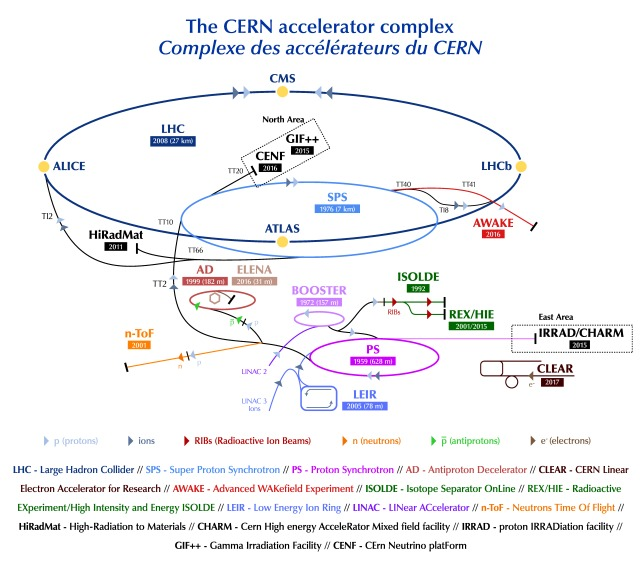
\includegraphics{CCC-v2018-print-v2.jpg}
\caption{The LHC is the last ring (dark blue line) in a complex chain of particle accelerators. The smaller machines are used in a chain to help boost the particles to their final energies and provide beams to a whole set of smaller experiments \cite{Mobs:2636343}.}
\label{fig:injection_chain}
\end{figure}

Before being injected into the \lhc, ion beams pass through a series of increasingly large accelerators, incrementally raising their energy \cite{Benedikt:2004wm}.
These lower-energy accelerators predate the \lhc and have each been used for many collision experiments throughout the history of CERN.
The CERN accelerator complex is sketched in \cref{fig:injection_chain}.

Protons are first collected by ionizing hydrogen gas, then accelerated to a kinetic energy of 50 \MeV\ by the Linac 2 linear accelerator.
The \ac{PSB} increases their energy to the relativistic level of 1.4 \GeV.
From there, the beam is energized in the \ac{PS} to 25 \GeV, then the \ac{SPS} to 450 \GeV.
These proton beams from the \ac{SPS} are used to fill the \lhc, where they are again accelerated to collision energies of a few \TeV each.

Lead ions are accelerated from rest by the Linac 3 linear accelerator, a dedicated ion \linac, to a kinetic energy of 4.2 \MeV per nucleon (\MeVn).
The \ac{LEIR} raises their energy to 72 \MeVn\ and also applies electron cooling to the ion beam.
This process involves merging the ions with an electron beam and allowing the mixture to come to thermal equilibrium so that the electron cloud absorbs thermal energy from the ions.
The ions are then re-separated from the electrons as they pass through a dipole magnet.
This cooling step, which effectively reduces the phase space volume of each bunch, is necessary to counteract the higher charge of the ions pushing them apart. %% equivalently, reducing the ``emittance'' of the beam
From the \ac{LEIR} the lead ion beam is injected into the PS, which raises its energy to 5.9 \GeVn, then the \ac{SPS}, which raises it to 177 \GeVn.
Finally, the beam is injected into the \lhc, where it is accelerated to a few \TeVn depending on the intended collision system.


\subsection{LHC main ring}

\begin{figure}[t]
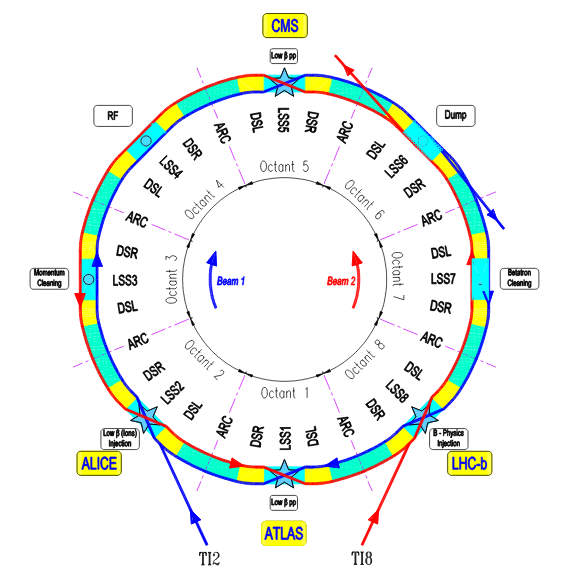
\includegraphics{LHC_schematic.png}
\caption{Schematic layout of the two beams of the \acs{LHC} \cite{Bruning:2004ej}.}
\label{fig:lhc_schematic}
\end{figure}

The \lhc ring does not trace a perfect circle, but is actually composed of eight alternating straight and curved arc sections through which pass two parallel beam pipes (\cref{fig:lhc_schematic}) \cite{Bruning:2004ej}.
The straight sections are each 528 m in length and contain the \rf cavities for acceleration, \acp{IP} for colliding beams at the various detector sites, and other features like injection spots and beam dumps.
The arc portions have a radius of curvature of $R = 2.8$ km and use a total of 1232 superconducting dipole magnets to turn the beams along the path.

The \rf cavities operate at 400 MHz, which corresponds to \rf buckets of 2.5 ns.
For ultra-relativistic beams, this corresponds to a minimum length spacing between bunches of 0.75 m.
Practically, however, the injection from the \ac{SPS} limits the bunch spacing to multiples of 25 ns, or 7.5 m separation.
The \lhc can thus fit a maximum of 3560 bunches in each of its rings, but they are not completely filled because gaps need to be left to allow safe beam dumps.
As of 2018, the smallest bunch spacing used for lead ions is 75 ns.

\begin{figure}[t]
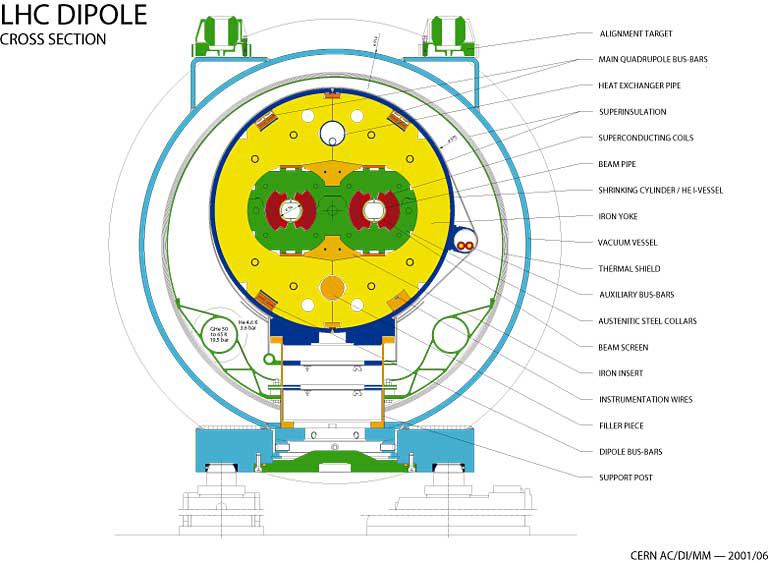
\includegraphics{LHC-PHO-2001-187.jpg}
\caption{A dipole magnet used to turn the beams along an arc. The two beams travel in the evacuated beam pipes running anti-parallel to each other, which requires the magnetic field in each to be opposite \cite{Valeriane:843195}.}
\label{fig:dipole_cross_section}
\end{figure}

The dipole magnets (\cref{fig:dipole_cross_section}) have a maximum design strength of 10 T, although the active field strength must remain proportional to the current energy of the beam fill.
For the \pPbenergy \pPb run they operated at 6.0 T with fully energetic beams.
In an asymmetric \pA beam configuration the beams must have different energies in order to trace out paths with the same magnetic field and radius of curvature.
They operate at fixed beam rigidity $|\mathbf{p}|/Ze \propto AEv/Z$ so that the per-nucleon energy for beams near the speed of light is proportional to $Z/A$.
To keep the beams focused, 392 quadrupole magnets are arranged in an alternating-polarity orientation.
This scheme alternately squeezes the beams horizontally and vertically, with a net effect of keeping the beam radius small.
Over 6000 additional multipole magnets are used for fine-tuning the magnetic fields.
The electromagnets use niobium-titanium (NbTi) as the conducting material, which has a critical temperature of 10 K and a maximum critical magnetic field of 15 T.
They are cooled with superfluid liquid helium (${}^{4}\textrm{He}$) to a temperature of 1.8 K.
A failure in the cooling system that allows the magnet temperature to rise above its critical temperature causes it to quench.
The increase in resistance from the loss of superconductivity causes a rapid temperature increase.
This is particularly disastrous if the helium is heated to its gaseous phase, causing it to explode\footnote{This actually occurred at the \lhc in September of 2008, delaying operations for over a year.}.


\subsection{LHC experiments}
The two largest \lhc experiments, ATLAS\footnote{an ``acronym'' for \textbf{A} \textbf{T}oroidal \textbf{L}HC \textbf{A}pparatu\textbf{S}} \cite{Aad:2008zzm} and CMS\footnote{\textbf{C}ompact \textbf{M}uon \textbf{S}olenoid} \cite{Chatrchyan:2008aa}, are general-purpose detectors that fulfilled one of their primary objectives with the joint discovery of the Higgs boson in 2012 \cite{HIGG-2012-27,Chatrchyan:2012xdj}.
They continue to be used in the search for physics beyond the Standard Model such as supersymmetry and large extra dimensions.
The large rapidity coverage of their calorimeter and tracking systems also make them highly capable of measuring both low- and high-energy probes of heavy ion collisions.
The ATLAS detector, which provided the data used in this thesis, is discussed in more detail in \cref{sec:atlas}.

Other than ATLAS and CMS, the \lhc houses a number of other experiments that are more specialized for specific purposes.
ALICE\footnote{\textbf{A} \textbf{L}arge \textbf{I}on \textbf{C}ollider \textbf{E}xperiment} \cite{Aamodt:2008zz} is a dedicated heavy-ion detector that is particularly adept at the identification of particle species.
With many subdetectors spread over a forward region from its \ac{IP}, the LHCb\footnote{\textbf{LHC b}eauty} experiment \cite{Alves:2008zz} can make detailed measurements of the decay products of b-quarks. Recently it has led to the observation of possible pentaquark states \cite{Aaij:2015tga}.
TOTEM\footnote{\textbf{Tot}al Cross Section, \textbf{E}lastic Scattering and Diffraction Dissociation \textbf{M}easurement at the LHC} \cite{Anelli:2008zza} has detectors in the forward region over 200 m on either side of the CMS \ac{IP}.
Its location near the beam pipe puts it in a position to detect the products of elastic and diffractive collisions, which are characterized by a lack of color connection that would otherwise produce particles in the mid-rapidity region.
The LHCf\footnote{\textbf{LHC f}orward} experiment \cite{Adriani:2008zz} has two detectors along LHC beamline at 140 m away from the ATLAS \ac{IP} on either side.
The latest experiment to join the ring is MoEDAL\footnote{the \textbf{Mo}nopole and \textbf{E}xotics \textbf{D}etector \textbf{A}t the \textbf{L}HC} \cite{Acharya:2014nyr}.
It is a mostly passive detector located next to LHCb, with the goal of direct detector of magnetic monopoles or other stable massive particles beyond the Standard Model.

\subsection{Dataset provided}

\begin{figure}[t]
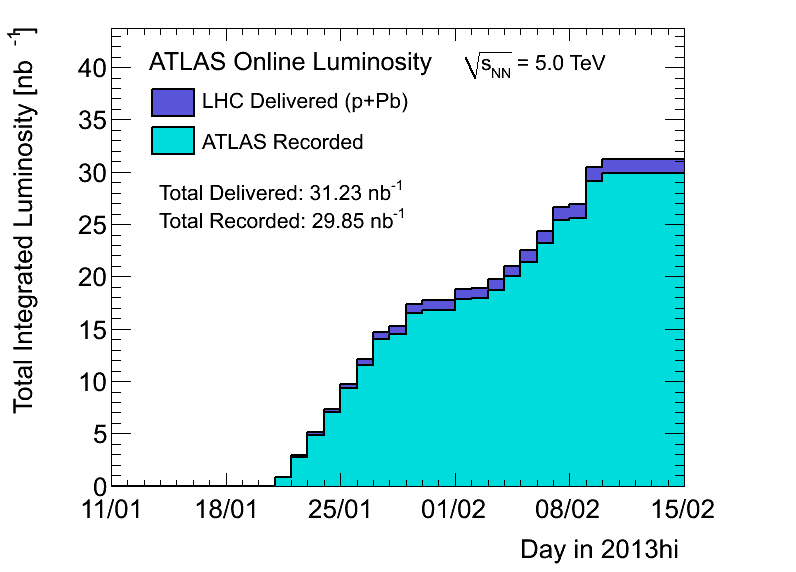
\includegraphics{sumLumiByDayUrgent.png}
\caption{The total integrated luminosity over the 2013 proton-lead data taking period.}
\label{fig:int_lumi}
\end{figure}

The results in this thesis use the 2013 \lhc \pPb dataset at a center-of-mass energy per nucleon of \pPbenergy.
%% In an asymmetric \pA beam configuration, 
The proton beam had an energy of 4 \TeV and the Pb ions had an energy per nucleon of $Z/A \cdot 4 \TeV = 1.57 \TeV$, so the center-of-mass of a proton and any one Pb nucleon had a longitudinal rapidity boost of $\ycm = 0.465$.
The \pPb run was divided into two periods between which the directions of the proton and lead beams were reversed to allow for better control over various systematic effects.
The maximum luminosity was $\Lumi_\textrm{peak} = 110 \times 10^{27} \, \textrm{cm}^{-2} \, \textrm{s}^{-1}$ over the 32 stable beam runs (16 in each period), though depending on the run $\Lumi_\textrm{peak}$ was as low as $22 \times 10^{27} \, \textrm{cm}^{-2} \, \textrm{s}^{-1}$.
The integrated luminosity of the data taking period from January 21 to February 10 is $\Lint = 28.1~\inb$ (\cref{fig:int_lumi}).
The bunch spacing of the beams was 200 ns, so the maximum bunch crossing rate was 5 MHz.

\section{The ATLAS detector}
\label{sec:atlas}

\begin{figure}[t]
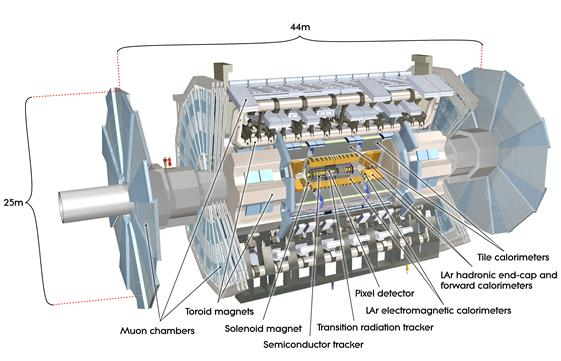
\includegraphics{ATLAS_layout.jpg}
\caption{The ATLAS detector and major subsystems \cite{Pequenao:1095924}.}
\label{fig:atlas_layout}
\end{figure}

The ATLAS experiment is a general purpose particle detector \cite{Aad:2008zzm} located at Point 1 on the \lhc ring, across the street from the main entrance to the CERN site at Meyrin, Switzerland.
Currently the largest volume accelerator detector in operation, it encompasses 44 m along the beam axis, has a diameter of 25 m, and weighs about 7 kilotonnes (\cref{fig:atlas_layout}).
Broadly speaking, the major subsystems of the ATLAS detector are (from inner- to outer-most): the \id, the magnet system, the calorimeters, and the muon spectrometer.
The muon spectrometer is essential for reconstructing a number of massive and exotic particles \cite{ATLAS:1997ad}; however, it will not be discussed in detail here as it is not used in the analyses presented in this thesis.
The extensive trigger and data acquisition system is also crucial for successful operation.
The \mbts detector sits on each side at a rapidity of $2.1 < |\eta| < 3.84$.
It is used to identify and trigger on minimum bias collisions.
The \zdc detectors are placed approximately 140 m on either side of the nominal \ac{IP} with a pseudorapidity of $|\eta| > 8.3$.
They are used to distinguish pileup events by detecting spectator nucleons that do not participate in the interaction.


\subsection{Magnets}
\label{subsec:atlas_magnet}

\begin{figure}[t]
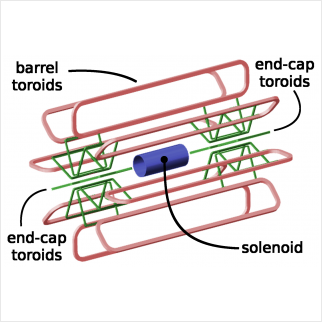
\includegraphics{atlas_magnets.png}
\caption{A schematic of the ATLAS magnet system.}
\label{fig:atlas_magnets}
\end{figure}

Two superconducting magnet systems are used to generate a large magnetic field with field lines parallel to the beam axis (\cref{fig:atlas_magnets}) \cite{ATLAS:1997ae}. %% tech design report
This magnetic field causes charged particles to follow a curved path through the detector, allowing their charge and transverse momentum to be measured according to \(  \pt = q B_z R\) where $R$ is the radius of curvature in the transverse plane.
A large solenoid 5.3 m in length and 2.3 m in diameter surrounds the ID and produces a 2 T magnetic field.
It is designed to produce as uniform of a magnetic field as is possible to allow precise measurements of the momentum of charged particles in the ID.
The toroid magnet system consists of 8 air-core coils in the barrel and two sets of 8 air-core toroids in each of the end-caps.
The magnetic field produced by these is non-uniform but bends charged particles outside of the ID for measurements by the muon spectrometer.

\subsection{Inner detector}
\label{subsec:atlas_id}

\begin{figure}[t]
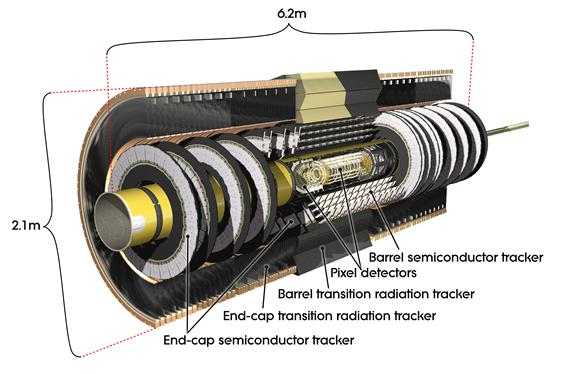
\includegraphics[width=0.57\linewidth]{id_whole.jpg}
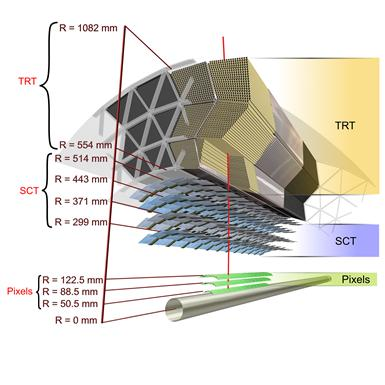
\includegraphics[width=0.42\linewidth]{id_slice.jpg}
\caption{Computer-generated images of the ATLAS inner detector. The left figure is a labeled graphic of the entire inner detector, and the right figure shows a cross-section of the barrel region \cite{Pequenao:1095926}.}
\label{fig:atlas_id}
\end{figure}

The ATLAS \id is designed to track the charged particles from collisions on their path from the beam pipe to the calorimeters, thereby inferring their charge and momentum \cite{ATLAS:1997ag,ATLAS:1997af,Aad:2010bx}.
It has a wide pseudorapidity coverage of \(\left| \eta \right| < 2.5\) and full azimuthal coverage in $\phi$.
The design resolution for the transverse momentum is \( \sigma_{\pt}/\pt = 0.05\% \, \pt /1 \GeV \oplus 1\% \), with a transverse impact parameter resolution of \( \sigma_{d_0} = 10 \mu\textrm{m}\) for tracks with a central rapidity.
Three sub-detectors are used, each in their own layer around the beam line.
From innermost to outermost, these are the silicon pixel detector, the \sct, and the \trt.


\subsubsection{Pixel detector}

The silicon pixel detector surrounds the beam pipe, covering radial distances from 50 mm to 150 mm, and is composed of 1744 silicon pixel modules \cite{Aad:2008zz}.
These are distributed over three concentric barrel layers and three disk layers on each endcap (\cref{fig:atlas_pixel}), so that the trajectory of a typical charged particle passes through three points in the pixel detector.
Each module is 16.4 mm by 60.8 mm and has 47 232 pixels of size 50 $\mu$m by 400 $\mu$m.
A total of 80.4 million readout channels are supported by 16 radiation-hardened front-end chips bump-bonded to each sensor.
A hit is recorded in each pixel when the signal exceeds a tunable threshold, and the time over threshold can be used to provide a measurement of ionization energy loss \dEdx used for particle identification.

\begin{figure}[t]
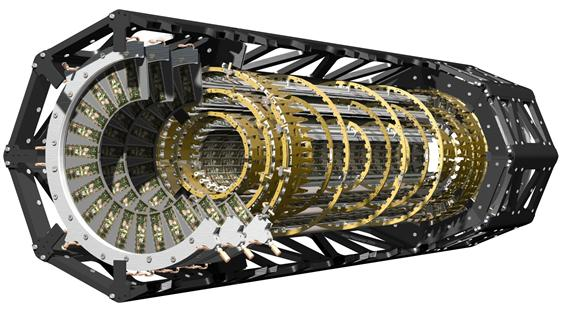
\includegraphics{pixel.jpg}
\caption{Computer-generated cutaway of the Pixel subdetector of the ATLAS inner detector \cite{Pequenao:1095925}.}
\label{fig:atlas_pixel}
\end{figure}


\subsubsection{Semi-conductor tracker}

The \sct consists of 4088 silicon-strip modules and covers a radial distance of 299 mm to 560 mm \cite{Aad:2014mta}.
These are placed in four concentric barrel layers and two endcaps of nine disks each.
A typical particle originating from the beam interaction region gets eight strip measurements in four space-points.
Most modules have four silicon-strip sensors, with two on each side glued back-to-back at a stereo angle of 40 mrad.
The relative angle between strips give space-points at the crossings.
The sensors are daisy-chained together to form 768 strips each with a length of 12 cm.
A total of 6.3 million readout channels are provided by radiation-hardened front-end readout chips.

\subsubsection{Transition radiation tracker}

The \trt covers the region from 563 mm to 1066 mm away from the beam line.
It consists of 298 304 proportional drift tubes (straws) each 4 mm in diameter \cite{Abat:2008zza}.
The straws are arranged in three cylindrical layers in the barrel region and are radially oriented in 80 wheel-like modules in the endcaps.
A typical track with $\pt > 0.5~\GeV$ and $|\eta| < 2.0$ crosses more than 30 straws.
There are a total of 350 848 readout channels.
The \trt hits are generally useful to refine the transverse momentum measurements of tracks seeded in the inner sub-detectors.

\subsection{Calorimetry}
\label{sec:atlas:calo}

\begin{figure}[t]
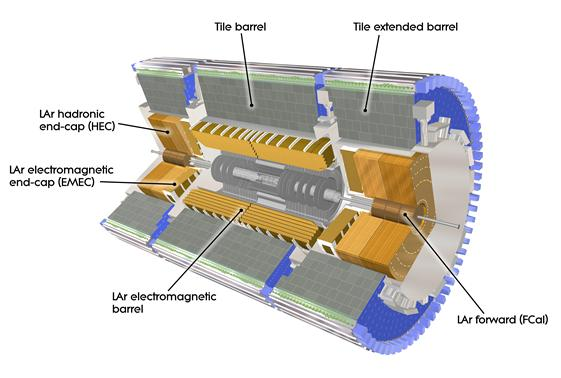
\includegraphics{calorimeter.jpg}
\caption{Computer-generated image of the ATLAS calorimeter systems \cite{Pequenao:1095927}.}
\label{fig:atlas_calorimeter}
\end{figure}

The ATLAS calorimetry system (\cref{fig:atlas_calorimeter}) covers nearly ten units of pseudorapidity at $|\eta| < 4.9$.
It provides measurements of high-energy particles by sampling the energy deposited in the calorimeters' dense active material \cite{Airapetian:1996iv}. %% performance tech design report
An absorbing material, placed in alternating layers with the active material, collects this energy from the showers.
ATLAS has two main categories of calorimeter, \emph{electromagnetic} and \emph{hadronic}.
The former is designed to induce \ac{EM} showers from electrons and photons, and the latter is designed to stop hadrons like protons and neutrons with both strong and \ac{EM} interactions.

\subsubsection{Electromagnetic calorimeter}

The electromagnetic calorimeter is the innermost calorimeter layer and covers the region $|\eta| < 3.2$.
It is divided into a barrel region at $|\eta| < 1.475$ and an end-cap at $1.375 < |\eta| < 3.2$, both of which use \ac{LAr} as an absorbing material \cite{ATLAS:1996ab} and lead as an active material. %% liquid argon
Electrons and positrons lose energy primarily through bremsstrahlung, radiating photons as they are slowed \cite{Fabjan:2003aq}.
Photons are stopped by the \ac{EM} calorimeter via pair production of electron-positron pairs.
A single electron or photon passing through the \ac{EM} calorimeter causes an electromagnetic cascade as these processes are repeated by product particles with progressively smaller energies.
As the energy is dispersed through the increasing number of shower particles, they are eventually slowed to a critical energy below which they interact through ionization and excitation, depositing their energy in the material.
The energy as a function of path length $\Delta l$ can be described by exponential decay \(E = E_0 e^{-\Delta l / X_0} \).
A typical photon or electron has a trajectory that, if extended beyond absorption, would cross a minimum of about 25 radiation lengths $X_0$ (\cref{fig:atlas_em_rad_length}).

\begin{figure}[t]
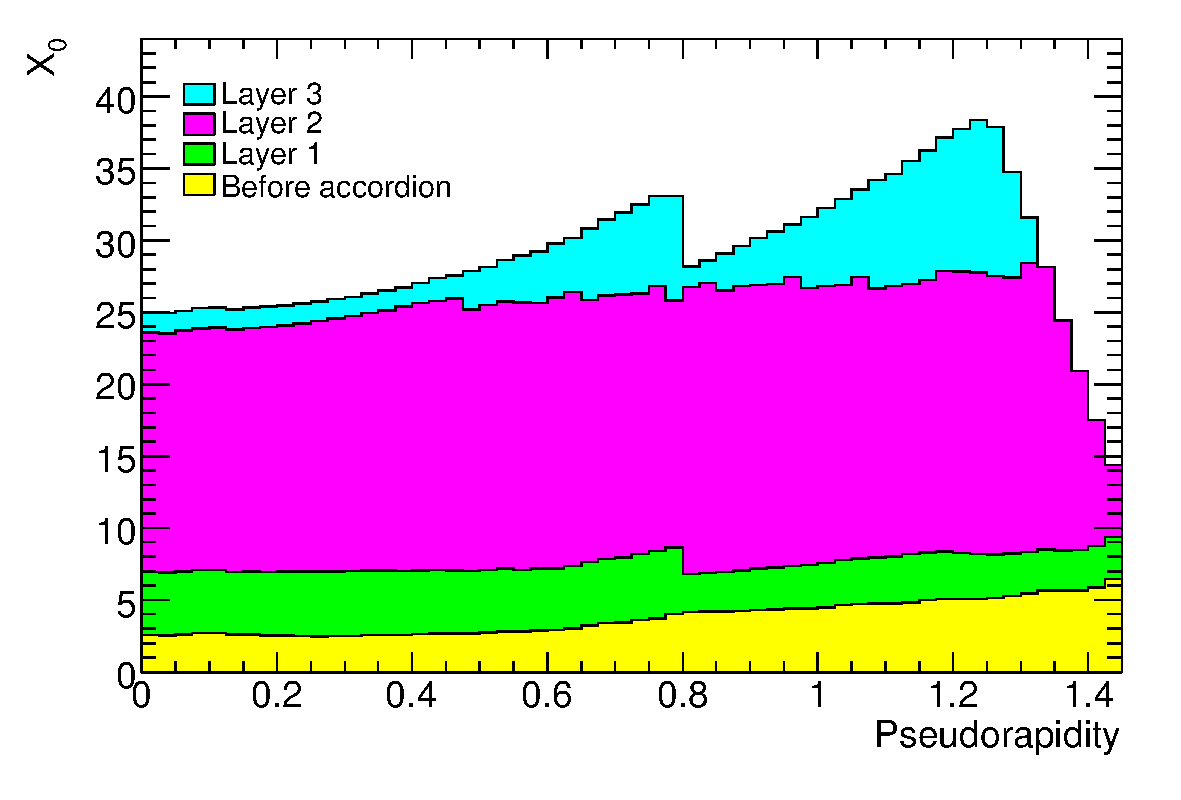
\includegraphics[width=0.49\linewidth]{x0_layers_barrel.pdf}
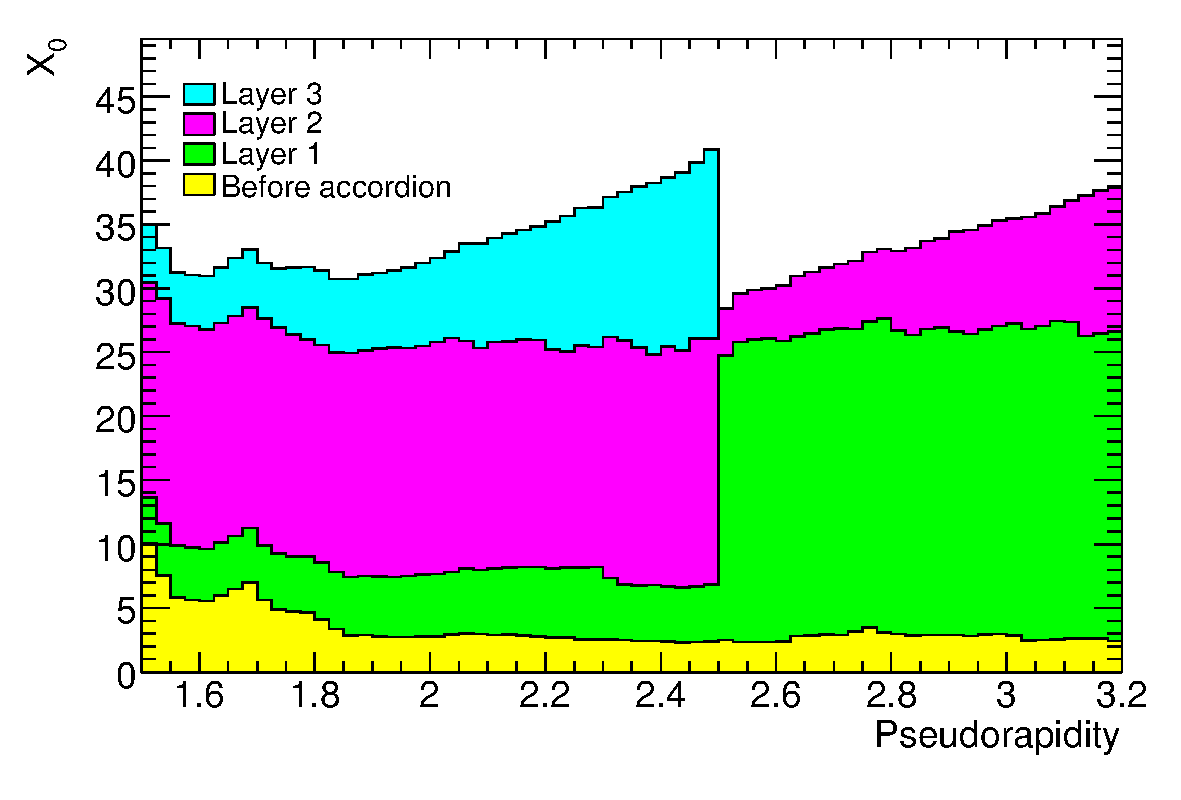
\includegraphics[width=0.49\linewidth]{x0_layers_endcap.pdf}
\caption{Thickness of the electromagnetic calorimeters in radiation lengths $X_0$ as a function of absolute pseudorapidity $|\eta|$ in the barrel (left) and end-cap (right) regions.}
\label{fig:atlas_em_rad_length}
\end{figure}

%% could talk about resolution following the Fabjan:2003aq ref

\subsubsection{Hadronic calorimeter}

The hadronic calorimeter lies outside the \ac{EM} calorimeter and is designed to stop protons and neutrons as well as the remnants of \ac{EM} cascades that are not completely absorbed by the \ac{EM} calorimeter.
The barrel region, along with the extended barrel region which encompasses the end-cap, cover $|\eta| < 1.7$ and comprise the tile system \cite{ATLAS:1996aa}.
The tile system does not use a \ac{LAr} active material, but rather is made of alternating steel plates and polystyrene scintillating tiles.
The \ac{HEC} detector covers $1.5 < |\eta| < 3.2$ and uses a \ac{LAr} active material with copper absorbers.
Most hadrons take a path that, if extended beyond the cascade, would cross at least 10 nuclear interaction lengths (\cref{fig:atlas_calo_nuclear_int_length}).

\begin{figure}[t]
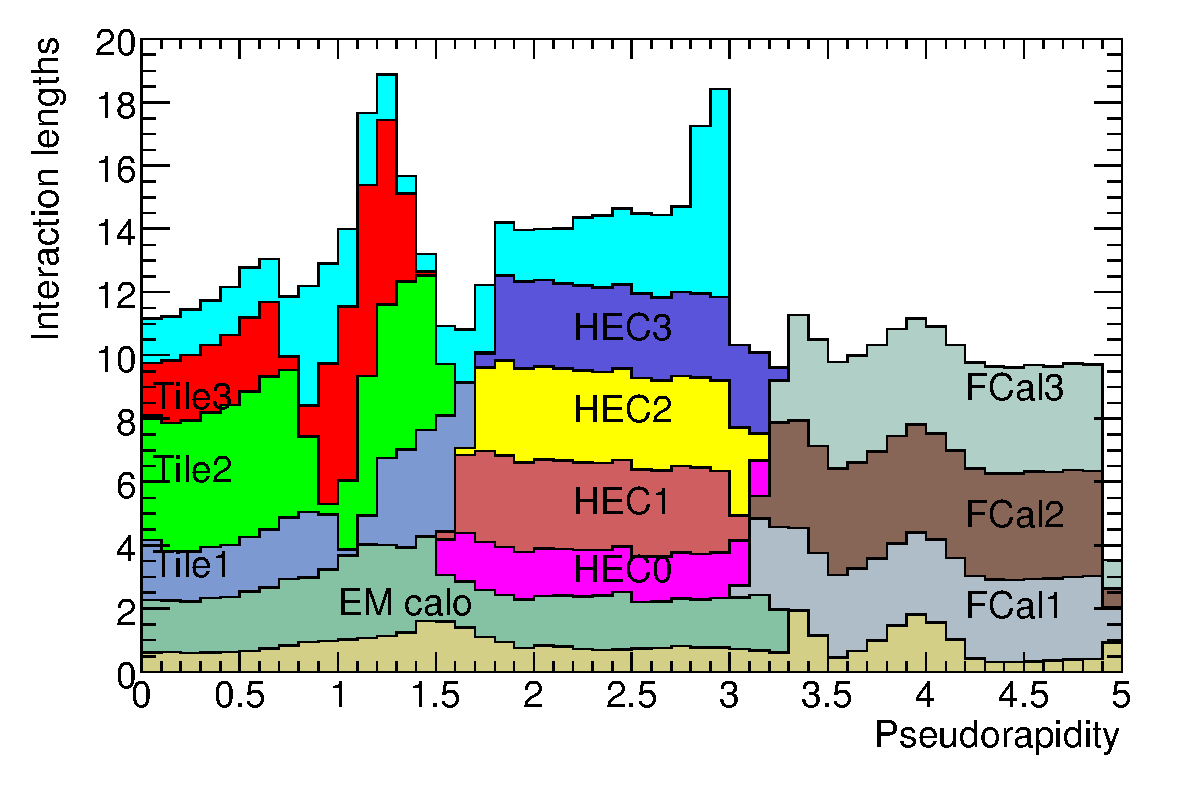
\includegraphics{calo_nuclear_int_length.pdf}
\caption{Nuclear interaction lengths for the combined ATLAS calorimetry system as a function of absolute pseudorapidity $|\eta|$.}
\label{fig:atlas_calo_nuclear_int_length}
\end{figure}

The hadronic cascade produced in the hadronic calorimeter is in some ways analogous to an \ac{EM} shower, though the interactions are mostly through the strong force.
Hadrons interact with the material and produce secondary particles that in turn produce their own shower, and energy is successively dispersed throughout the products.
The relative complexity of hadronic and nuclear processes makes a precise description more difficult since there are a greater number of relevant particles and nuclear resonances.
Sophisticated \mc simulations, using detailed models of the nuclear interactions, are required to accurately describe the physics of hadronic calorimeters.

\subsubsection{Forward calorimeter}
The \fcal consists of three layers situated underneath the endcap calorimeters at $3.1 < |\eta| < 4.9$.
It uses \ac{LAr} as its active material.
The first layer is designed for electromagnetic calorimetry and uses copper as its absorbing material, while the remaining two layers at larger $|z|$ are intended primarily for hadronic calorimetry and use tungsten as their absorbing material.
Due to its location in the forward region near the beam pipe the \fcal receives a greater amount of radiation than the other calorimeters.
In heavy ion collisions the \fcal is useful for measuring the centrality and reaction plane of events.

\subsection{Trigger}
%% \subsection{Trigger and data acquisition systems} %% maybe we don't need to get into DAQ
\label{subsec:atlas_trigger} % is it even worth labeling these if they're not numbered?

%% 200 ns for Pb; low mu reduces collisions
The \lhc can deliver a bunch crossing as often as the bunch spacing time, which was 200 ns for the \pPb run but can be as rapid as 25 ns for \pp collisions.
It is infeasible to record full events at the corresponding rate of up to 40 MHz, and many of the bunch crossings have cosmic backgrounds, out-of-time pileup\footnote{The \lhc \rf has a frequency of 2.5 ns, but the timing is designed to only fill a bunch every 25 ns. Stray particles can still find their way into unintended \rf buckets, causing out-of-time pileup when they collide at the \ac{IP}.}, or no collision at all.
Therefore the ATLAS trigger system needs to be capable of rapidly evaluating whether the data from an event is worth recording \cite{Aad:2012xs}. %% reference to performance paper
The trigger system has three levels, each of which processes the data and filters events for the next level.

The \ac{L1} trigger is a low-level hardware system that makes rapid determinations based on activity in the calorimeters, \mbts, \zdc, and muon spectrometers \cite{ATLAS:1998ad}.
It uses parallel data pathways separate from the regular readout path, with electronics optimized for speed over precision.
The \ac{CTP} combines the \ac{L1} trigger signals into combinations of \ac{L1} bits which are used to seed the \ac{L2} trigger.

The software-based \ac{HLT} is composed of the remaining two trigger levels, the \ac{L2} trigger and \ac{EF} \cite{ATLAS:2003aa}.  %% high-level trigger and DAQ
The \ac{L2} trigger uses regions of interest determined by the \ac{L1} trigger to seed algorithms that perform a more precise evaluation of the events.
The items from the \ac{L2} trigger processing are passed to the \ac{EF}, which uses the full offline readout path in order to mitigate biases from the ultra-fast \ac{L1} response.
An event is potentially recorded if it is selected by a trigger chain, which is defined by a \ac{L1} seed with \ac{HLT} items.
Recording every event that satisfies a trigger chain would still overwhelm the data acquisition system.
Prescales can be applied for items at any level in a trigger chain.
A trigger item with a prescale of $N$ is only flagged to be recorded at every $N$th instance of the trigger item firing.
The prescales of each trigger item are adjusted based on the physics goals of the run.

While many analyses of high energy data focus on the behavior of exceptional or rare events, the results presented in this thesis are concerned primarily with \minbias events.
The physics of interest is the bulk dynamics of the events on average rather than jets or rare particle decays.
General high-multiplicity and high-transverse-energy triggers are used to supplement the size of the data sample for central events.
These triggers are only used in the regime where their efficiency is practically 100\%, so the details of their performance are not as crucial here as they might be elsewhere.
